 \documentclass[12pt]{article}
\usepackage[T2A]{fontenc}
\usepackage[utf8]{inputenc}       

\usepackage[english]{babel}
\usepackage{amsmath,amsfonts,amsthm,amssymb,amsbsy,amstext,amscd,amsxtra,multicol}
\usepackage{verbatim}
\usepackage{tikz}
\usetikzlibrary{automata,positioning}
\usepackage{multicol}
\usepackage{graphicx}
\usepackage[colorlinks,urlcolor=blue]{hyperref}
\usepackage[stable]{footmisc}
\usepackage{ dsfont }
\usepackage{wrapfig}
\usepackage{xparse}
\usepackage{ifthen}
\usepackage{bm}
\usepackage{color}
 \usepackage{subfigure}
 
\usepackage{algorithm}
\usepackage{algpseudocode}

\usepackage{xcolor}
\usepackage{hyperref}
\definecolor{linkcolor}{HTML}{799B03} % цвет гиперссылок
\definecolor{urlcolor}{HTML}{799B03} % цвет гиперссылок
 
%\hypersetup{pdfstartview=FitH,  linkcolor=linkcolor,urlcolor=urlcolor, colorlinks=true}

\newtheorem{theorem}{Theorem}[section]
\newtheorem{lemma}{Lemma}[section]

\DeclareMathOperator{\sign}{sign}
\DeclareMathOperator{\grad}{grad}
\DeclareMathOperator{\intt}{int}
\DeclareMathOperator{\conv}{conv}
\begin{document}

\tableofcontents
\newpage

We consider some new approach to method convex 2-dimensional optimization on a fixed square recently proposed by Yu. E. Nesterov (see ex.1.5 in https://arxiv.org/pdf/1711.00394.pdf). The method can be interested for to solve a dual problem for a convex problem with two functional constraints. The idea of the method consists in the narrowing of the domain until we achieve an acceptable quality of the solution. This method has to search minimum on the separating segments and we propose some non-depended on required accuracy stop condition for it. Estimations for the iterations number are proved for the cases of smooth and non-smooth functions. Besides there is an experimental comparison of our method with other inexact methods of convex optimization such as ellipsoid method with epsilon-subgradient and primal and fast gradient method with delta-L-oracle. The experiments were made on dual problems for problems with two constraints As a result, our method with provided in this work strategy has the best result.

\section{Introduction}

In this paper we research one method of optimization on a square in $\mathbb{R}^2$. The method was offered by Nesterov (see ex.~4 from ~\cite{task}). interested for to solve a dual problem for a convex problem with two functional constraints. This method is reffered as Halving Square Method. 

 The idea of the method consists in the narrowing of the domain until we achieve an acceptable quality of the solution. This method has to search minimum on the separating segments. In the next section there is description of method and pseudocode for it.

In the paper~\cite{Ston_Pas} there are some results for this method. Namely, there is an estimate for iterations number. Additionally, the authors provided strategy for subproblem on segment. Also there are comparison of this method with method of ellipsoids. Discussed method showed better results on time.

But the provided strategy has several disadvantages. Firstly, the required accuracy for the problem on segment significantly depends on the required accuracy for initial task on segment. It is essential disadvantage when one want to solve initial task extra accurately. Secondly, the method has convergence only on function and is able to not converge to solution on argument.

In this paper we continue this research and provide a new strategy for separating segments. According to it there is stop condition for one-dimensional problem. This stop condition does not depend on required initial accuracy and the HSM with this strategy converges to the solution on argument. The discussion of this strategy is in the section \ref{Delta}.

Moreover, the new estimates for iterations number was provided in this work. There are estimates for smooth and non-smooth problem when on each iteration one chooses rectangle that include the global solution. Additionally, there are theoretical and experimental comparisons of this estimates.

Also we carried out some numerical expirements for to compare the Halving Square Method with other methods. Firstly, it is comparison of different strategies for the Halving Square Method on problems when we can calculate object function's value analitacally. Secondly, it is comparison on dual problem when we can not do it. In this case we compare our method with other such inexact methods as primal gradient method, fast gradient method and ellipsoid method.

This experiments showed that the Halving Square Method with provided in this work strategy is optimal method for to solve dual problem with high accuracy. And the gain of using this method grows with the growth of required accuracy.

\section{Method Description}

Let's consider a following task:

$$\min_{(x,y)}\left\{f(x,y)|(x,y) \in Q\right\},$$
where $f$ is a convex function, $Q$ - is a square on the plane.

Let's consider a following method. One solves task of minimization for a function $g(x) = f\left(x, y_0 = \frac{a}{2}\right)$ on a segment $[0, a]$ with an accuracy $\delta$ on function. After that one calculates a subgradient in a received point and chooses the rectangle which the subgradient "does not look" in. Similar actions are repeated for a vertical segment. As a result we have the square decreased twice. Let's find a possible value of error $\delta_0$ for task on segment and a sufficient iteration's number $N$ to solve the initial task with accuracy $\epsilon$ on function.

Let's describe an algorithm formally. See pseudo-code \ref{alg:Example}.

\begin{algorithm}[H]
\caption{Halving Square Method}\label{alg:Example}
\begin{algorithmic}[1]
\Function{Method}{convex function $f$, square $Q = [a, b]\times[c,d]$}

$x_* \leftarrow \arg\min_{x\in[a,b]}f(x, \frac{c+d}{2})$
 
$g \leftarrow \partial f(x_*, \frac{c+d}{2})$
 
\If{g[1] > 0}
\State$Q := [a,b] \times [c, \frac{c+d}{2}]$ 
\Else
\State$Q := [a,b] \times [\frac{c+d}{2}, d]$ 
\EndIf

 $y_*\leftarrow \arg\min_{y\in[c,d]}f(\frac{a+b}{2}), y) $
 
 $g \leftarrow \partial f(\frac{a+b}{2}), y_*)$
 
 \If{g[0] > 0}
 \State$Q := [a, \frac{a+b}{2}] \times [c, d]$ 
\Else
\State$Q := [\frac{a+b}{2},b] \times [c, d]$ 
\EndIf
\If{$f(\frac{a+b}{2}, \frac{c+d}{2})-f^*>\epsilon$}
\State Method($f$, $Q$) 
\EndIf

\Return$(\frac{a+b}{2}, \frac{c+d}{2})$
\EndFunction 
 \end{algorithmic}
\end{algorithm}

The $\arg\min$ will be find through dichotomy method that uses derivative, i.e. it is method that take the derivative in the center of curent segment and select the part segment that anti-gradient looks at. The interesting remark is that it is one-dimensional analog of our method. 

The sufficient accuracy for $\arg\min$ will be discussed in the section \ref{Delta}.

\section{Algorithm correctness}

In this section there are profes for the fact that our method works for some accuracy for one-dimensional problem on segment.

Now we introduce the following notation. If we solve the one-dimensional problem then $f_\perp'$ is a perpendicular to the segment subgradient's component, i.e. it is a derivative on the variable that is fixed on this segment. In this case $f'_\parallel$ is a parallel to the segment subgradient's component.

We will use the following enough obvious lemma.

\begin{lemma}
\label{subgradient}

If $\textbf{x}_*$ is a solution of one-dimensional problem on a horizontal segment then

$$\exists g \in \partial f(\textbf{x}_*) : g_\parallel = 0$$
\end{lemma}
\begin{proof}
...
\end{proof}

\begin{theorem}
Let's the $f$ has continuous derivative on the square. Then there is a neighbourhood of a solution of optimization task on segment such as a choice of rectangle will not change if one use any point from the   neighbourhood.
\end{theorem}
\begin{proof}
...
\end{proof}

The method does not work for all convex functions even for zero error on segment. There is an example of non-smooth convex problem in \cite{Ston_Pas} when this method can not converge to the solution more accurately then one constant.

\section{One-Dimensional Problem}
\label{Delta}

In this section we describe a sufficient conditions for to stop to solve one-dimensinal problem on segment. We will use the following notation:

$$(x_*,y_*)\text{ -- solution of one-dimensional problem} $$
$$\delta = |x-x_*| \text{ -- distance}$$

In the work \cite{Ston_Pas} there are proves for the following theorem:

\begin{theorem}
\label{ConstEst}
Let $f$ be convex $M$-Lipschitz continious function with $L$-Lipschitz continious gradient.
Then if each one-dimensional task was solved with the following accuracy
\begin{equation}
\delta \leq \frac{\epsilon}{2Ma(\sqrt{2}+\sqrt{5})(1-\frac{\epsilon}{La\sqrt{2}})}
\end{equation}
then this method converge to minimum of $f$ on square with accuracy $\epsilon$ on function.
\end{theorem}

This strategy requires to solve each one-dimensional problem with accuracy of order of $\epsilon$. It can be sufficient disadvantage for iterations on the big segments in the start of method's work. Also this strategy does not give convergence on argument. We will call this strategy \textbf{ConstEst}(Constant Estimate).

Let's develop strategy where there is convergence on argument. Rectangles are defined correctly for a horizontal optimization task, if:

\begin{equation}\label{MCH}
f'_y(\textbf{x}_*)f'_y(x_*+\delta, y_*) > 0
\end{equation}

Analogically, for a vertical segment:
\begin{equation}\label{MCV}
f'_x(\textbf{x}_*)f'_x(x_*, y_*+\delta) > 0
\end{equation}

\begin{theorem}
\label{CurGrad}
Let function $f$ be convex and has $L$-Lipschitz continuous gradient and a point $\textbf{x}_*$ is a solution of optimization's  task on a current segment. 

The current segment is horizontal and $M = |f_y'(\textbf{x}_{current})|$ or the current segment is vertical and $M = |f_y'(\textbf{x}_{current})|$. Then rectangle is defined correctly if a distance between $\textbf{x}_{cur}$ and accurate solution on segment is less than $\frac{M}{L}$.
\end{theorem}
\begin{proof}
Condition \eqref{MCH} is met if there is a derivative $f'_y(x_0+\delta, y_0)$ in a neighbourhood of 
$f'_y(\textbf{x}_*)$ with radius $\left|f'_y(\textbf{x}_{cur})\right|$:

$$\left|f'_y(\textbf{x}_*) - f'_y(\textbf{x}_{cur})\right|<\left|f'_y(\textbf{x}_{cur})\right|$$

The $L$-Lipschitz continuity gives following inequality:

$$\left|f'_y(\textbf{x}_*) - f'_y(\textbf{x}_{cur})\right| \leq L|\delta|$$

Therefore the following possible value is sufficient to select rectangle correctly:

$$\delta_0 < \frac{M}{L} \leq \frac{\left|f'_y(\textbf{x})\right|}{L}$$

Statement for vertical segment is proved similarly.
\end{proof}

Theorem \ref{CurGrad} gives stop conditions in the case when gradient in point-solution on segment and close points is large. But what should we do if gradient in this point is small?

\begin{theorem}
\label{small}
Let $f$ be $M$-Lipschitz continuous convex and have $L$-Lipschitz continuous gradient. The points $\textbf{x}_*$ is one-dimensional problem's solution and $\textbf{x}$ is its approximation, $\delta = \|\textbf{x}_*-\textbf{x}\|$ is a distance between them.

Then for accuracy on function $\epsilon$ following condition in point $\textbf{x}$ is sufficient:
$$\delta \leq \frac{\epsilon-LR|f_\perp'(x_*)|}{L+MR}, $$
where $R=a\sqrt{2}$ is size of current square.
\end{theorem}

\begin{proof}

From the lemma \ref{subgradient} we have:

$$g \in \partial f(\textbf{x}_*): g_\parallel = 0.$$

Then the following inequallity is true by diffenition of subgradient:

$$f(\textbf{x}^*) - f(\textbf{x}_*) \geq (g, \textbf{x}^* - \textbf{x}_*)$$

Using  Cauchy–Bunyakovsky–Schwarz inequality one has following inequality

$$f(\textbf{x}_*) - f(\textbf{x}^*) \leq -(g, \textbf{x}^* - \textbf{x}_* )\leq$$
$$\leq \|g\| \|\textbf{x}^* - \textbf{x}_*\|\leq \|g\|a\sqrt{2}$$

On the other hand, we have:

$$f(\textbf{x})-f(\textbf{x}_*)\leq M\delta$$

Therefore we have the following estimate:

$$f(\textbf{x})-f(\textbf{x}^*) \leq M\delta +\|g\|a\sqrt{2} = M\delta + |f_\perp'(\textbf{x}_*)|R$$

From Lipschitz continious from gradient we have:

$$f(\textbf{x})-f(\textbf{x}^*) \leq M\delta + \left(|f_\perp'(\textbf{x})|+L\delta\right)R$$

Then for to approach accuracy $\epsilon$ at the point $x$ the following condition is sufficient:

$$M\delta +\|g\|a\sqrt{2} = M\delta + \left(|f_\perp'(\textbf{x})|+L\delta\right)R \leq \epsilon$$

$$\delta \leq \frac{\epsilon - |f_\perp'(\textbf{x})|}{M+LR}$$
\end{proof}

Then our addaptive strategy is following. One is to calculate untill the following condition is met:

\begin{equation}
\label{Adaptive}
\delta \leq \max\left\{
	\frac{|f_\perp'(\textbf{x})|}{L}, 
	\frac{\epsilon - |f_\perp'(\textbf{x})|}{M+LR}
	\right\}.
\end{equation}

And if the condition from theorem \ref{small} we stop our method. This strategy is reffered as \textbf{CurGrad}(Current Gradient).


Let's make a couple of remarks.

Firstly, we can replace the Lipschitz condition on the square by the Lipschitz condition on the segments in the written above theorems.

Secondly, we can use in this theorems Lipschitz constants not for gradients but for partitial derivative on segments. Its proves are obvious enough and almost repeat proves for this theorem.


\section{Convergence}

Below proved estimates are correct if each iterations was correct, i.e. after each iteration there is the solution in the selected rectangle. It is important condition

\begin{theorem}
If function $f$ is convex and $L_f$-Lipschitz continuous, then for to solve initial task with accuracy $\epsilon$ on function one should make following iteration's numbers:
\begin{equation}\label{NI1}N = \left\lceil\log_2\frac{\sqrt{2}L_fa}{\epsilon}\right\rceil\end{equation}
where $a$ is a size of the initial square $Q$.
\end{theorem}

\begin{proof}
The square's size equals $\frac{a}{2^k}$ on $k$'th iteration. If each irerations was correct then
$$\|\textbf{x}_k-\textbf{x}^*\|\leq \frac{a}{2^k}\sqrt{2}$$
Using the fact that function is Lipschitz continuous we have estimate \ref{NI1}
\end{proof}

The similar estimate was proven for the fist strategy without convergence on argument too. This proof can be found in the work \cite{Ston_Pas}.

There are functions which estimates from written above theorem are very accurate for.

\textbf{Example 5.} Let's consider following task with positive constant $\alpha$:

$$\min\left\{\alpha(x+y)|Q = [0,1]^2\right\}$$

If one take a center of a current solution as approximate  solution one have value $\frac{\alpha}{2^N}$ after $N$ iterations. Therefore, for accuracy $\epsilon$ one has to $\lceil\log_2\frac{\alpha}{\epsilon}\rceil$. For this function $L_f = 2\alpha$. Therefore, estimate \eqref{NI1} is accurate for such tasks with little error that not more one iteration.


We can improve written above estimates if to add new conditions:

\begin{theorem}
Let function $f$ be convex.

If

1. Function $f$ has $L$-Lipschitz continious gradient

2. $\exists \textbf{x}^*\in Q: \nabla f(\textbf{x}^*) = \textbf{0}$

3. Strategy gives a convergence on argument

then for to approach accuracy $\epsilon$ on function the following iterations number is sufficient:
\begin{equation}\label{NI3}N = \left\lceil\frac{1}{2}\log_2\frac{Ma^2}{4\epsilon}\right\rceil,
\end{equation}
where $a$ is a size of the initial square $Q$.
\end{theorem}

\begin{proof}
For all convex functions there is following inequality (one may find proof in \cite{Nesterov}):
$$f(\textbf{x}) - f(\textbf{x}^*) - (f'(\textbf{x}^*), \textbf{x} - \textbf{x}^*) \leq \frac{L}{2}\|\textbf{x}-\textbf{x}^*\|^2$$

If $\textbf{x}^*$ is a solution and an internal point, then $f'(\textbf{x}^*) = 0$:

$$f(\textbf{x}) - f(\textbf{x}^*)\leq \frac{L}{2}\|\textbf{x}-\textbf{x}^*\|^2$$

After $N$ iterations we have the estimate:

$$f(\textbf{x}) - f(\textbf{x}^*)\leq L\left(\frac{a}{2^N}\right)^2$$

Using it we have estimate \eqref{NI3}.
\end{proof}

Estimate \ref{NI1} works in all cases and better then estimate \ref{NI3} when following condition is met:

$$\frac{2L_f^2}{L_g}\leq \epsilon,$$
where $L_f, L_g$ is Lipschitz constants for function and for gradient. On the other hand, the estimate \ref{NI3} works if point with zero gradient exists in the square. 


\section{Halving Cube Method}

This Halving Square Method is optimization method for convex problem on square. But there is obvious generalization for convex problems in high dimensional spaces on $n$-dimensional hypercube.  Let's describe it:

1. Take $(n-1)$-dimensional hyperplane in hypercube that includes hypercube center and is parallel to one of its face.

2. To solve optimization problem on this set with accaracy that is met to condition from theorem \ref{CurGrad}.

3. Calculate gradient in this point and select rectangle which antigradient look into.

4. Repeat the third step $n$ times for each hyperplane in hypercube that includes hypercube center and is parallel to one of its face.

5. Repeat the previous step until required accuracy is achieved.

The proves for convergence for smooth function and for strategy repeat proves in the case of 2-dimensional space. Moreover, obvious enough that the following theorems are correct when on the fourth algorithm step rectangle was selected correctly.

\begin{theorem}
If function $f$ is convex and $L_f$-Lipschitz continuous, then for to solve initial task with accuracy $\epsilon$ on function one should make following iteration's numbers:
\begin{equation}N = \left\lceil\log_2\frac{\sqrt{n}L_fa}{\epsilon}\right\rceil\end{equation}
where $a$ is a size of the initial square $Q$.
\end{theorem}

\begin{theorem}
Let function $f$ be convex.

If

1. Function $f$ has $L$-Lipschitz continious gradient

2. $\exists \textbf{x}^*\in Q: \nabla f(\textbf{x}^*) = \textbf{0}$

3. Strategy gives a convergence on argument

then for to approach accuracy $\epsilon$ on function the following iterations number is sufficient:
\begin{equation}N = \left\lceil\frac{1}{2}\log_2\frac{Ma^2}{4\epsilon}\right\rceil,\end{equation}
where $a$ is a size of the initial square $Q$.
\end{theorem}

Note the hyperplane in hypercube in the first step is $(n-1)$-dimensional hypercube. And we can use for it this method too. So, we solve the convex problem on $n$-dimensional hypercube recursively.

But this method has two essential disadvanteges for enough high dimensional spaces. Fisrtly, the required iterations number depend on logarithm of dimension. Of course, it is essential only for very high dimensional problems. Secondly, recursive algorithm will be extra slow because each the complexity of each iteration for this method is factotial of dimension.

We don't expect inspired result for each modification and we will not test it.

\section{The Dual Problems}
\label{details}

This method is interesting for to solve dual problems for problems with two constraints. Namely, we are interesting in solution of the following problem:

\begin{gather}
\phi(\lambda_1, \lambda_2) \rightarrow \min_{\lambda\geq 0},\\
\text{where } \phi = -\min_\textbf{x}\left(f(\textbf{x}) + \lambda_1 g_1(\textbf{x}) + \lambda_2 g_2(\textbf{x})\right)
\end{gather}
$$\textbf{x}(\lambda) = \arg\min_\textbf{x}\Phi(\textbf{x}, \lambda)$$

In this section we will discuss how transform this task to task of the task of minimization on square, what is derivative and lipschitz constants. Also, there is description of way for to calculate the value of function $\phi$ and its derivative.

Fitstly, let's transform this problem to the problem of minimization on square. According to \cite{task} (see ex. 4.1), we can add following restraint for the dual variables:

\begin{gather}
\label{restr:dual}
\|{\lambda}\|_1 \leq a = \frac{1}{\gamma}\left(f(\overline{\textbf{x}}) -\min\limits_{\textbf{x}}f(\textbf{x})\right),\\
\text{where $\overline{\textbf{x}}:g_i(\overline{\textbf{x}})<0,\gamma = \min\limits_i[-g_i(\overline{\textbf{x}})]$}
\end{gather}
According to this statemant ther is the $\lambda^*$ in square $Q = [0, a]^2$. And we have following optimization task:
\begin{gather}
\label{dual}
\phi(\lambda_1, \lambda_2) \rightarrow \min_{\lambda \in Q}
\end{gather}

The next point is a gradient of function $\phi$. It will be calculated according to well-known Demyanov-Danskin-Rubinov Theorem, see \cite{DDR-theorem}.

\begin{theorem}
Let $\phi(\lambda)=\min\limits_{x\in X}\Phi(x,\lambda)$ for all $\lambda\geq0$, where $\Phi$ is a smooth convex function with respect to $\lambda$ and $x(\lambda)$ is the only maximum point. Then
$$\nabla \phi(\lambda) = F'_\lambda\left(x(\lambda),\lambda\right)$$
\end{theorem}

If theorem's conditions is met for our case then we have derivative value:

\begin{equation}
\phi'_{\lambda_k}(\lambda) = g_k\left(\textbf{x}(\lambda)\right)
\end{equation}

Additionally, we need a Lipschitz constant for gradient. In the work \cite{Stonykin} there is following theorem:
\begin{theorem}
Let $f(x)$ be a $\mu_f$-strongly convex function, the function $g(x)$ satisfies the Lipschitz condition with a constant $M_g$. Then the function $\phi(\lambda) = \min_\textbf{x}\left(f(\textbf{x}+\lambda_1g_1(\textbf{x}) + \lambda_2g_2(\textbf{x})\right)$ defined in \ref{phi}, where $x(\lambda) = \arg\min\limits_x(f(x)+\lambda g(x))$, has Lipschitz smooth gradient with constant $L_{\phi'} = \frac{M_g^2}{\mu_f}$
\end{theorem}

This theorem can be proved easy for the 2-dimensional space. In this case $g$ is a vector-function.

The next subsections are devoted to efficient calculation of function's and derivative's values.

The main problem for such saddle-points problems is that one can not calculate $\textbf{x}(\lambda)$ presicely. Therefore, one have not precise value of the gradient in our method.

We need $\textbf{x}(\lambda)$ when we solve one-dimensional problem. There are three following cases:

1. The step of dichotomy on segment.

2. The test of stop-condition.

3. The select of rectangle.

Let's assume that we solve one dimensional problem on segment that is paralell to the first axis. For the case of the second axis the results will be similar. In the each above written case we are interesting in not full gradient but :

1. The first component, i.e. $g_1(\textbf{x}(\lambda))$.

2. (for the strategy through current gradient) the value of difference $\delta-\frac{|g_2(\textbf{x}(\lambda))|}{L}$, where $L$ is a Lipschitz constant for gradient of $\phi$.

3. The second component, i.e. $g_2(\textbf{x}(\lambda))$.

Moreover, for each case only sign of corresponding expression. For it we will use the following lemma.
\begin{lemma}
$\forall a,b\in\mathbb{R}:b\neq 0, |a-b|\leq |b| \Rightarrow \sign a = \sign b$
\end{lemma}
\begin{proof}
If $b>0$ and $a\leq b$ then the lemma's condition is equivalent to the following condition:
$$b-a\leq b\Rightarrow a\geq 0.$$
If $b>0$ and $a \geq b$ then $a\geq 0$.

The case of negative $b$ is proven similary.
\end{proof}

According this lemma we have the following stop conditions for calculating $\textbf{x}(\lambda)$ for the cases:

1. $|g_1(\textbf{x})-g_1(\textbf{x})|\leq |g_1(\textbf{x})|$

2. $\frac{1}{L}\Big||g_2(\textbf{x})|-|g_2(\textbf{x}(\lambda))|\Big|\leq \Big|\delta-\frac{|g_2(\textbf{x})|}{L}\Big|$

3. $|g_2(\textbf{x})-g_2(\textbf{x}(\lambda))|\leq |g_2(\textbf{x})|$

In this moment we can state the following theorem.

\begin{theorem}\label{x_lambda}
Let $g_k$ be $L_{g_k}$-Lipschitz continious. Then the following statements are true:

1. For to make the dichotomy step correctly one can calculate $\textbf{x}(\lambda)$ untill the following condition is approached:
$$L_{g_1}\|\textbf{x}-\textbf{x}(\lambda)\|\leq |g_1(\textbf{x})|.$$

2. For to test stop condition correctly one can calculate $\textbf{x}(\lambda)$ untill the following condition is approached:
$$\frac{L_{g_2}}{L}\|\textbf{x}-\textbf{x}(\lambda)\|\leq\Big|\delta-\frac{|g_2(\textbf{x})|}{L}\Big|,$$
where $\delta$ is a distance between $\lambda$ and solution of one dimensional task $\lambda_*$.

3. For to select rectangle according to strategy one can calculate $\textbf{x}(\lambda)$ untill the following condition is approached:
$$L_{g_2}\|\textbf{x}-\textbf{x}(\lambda)\|\leq |g_2(\textbf{x})|.$$
\end{theorem}

There are two interesting remarks.

Firstly, the calculating of $\textbf{x}(\lambda)$ does not depend on required accuracy $\epsilon$ for function $\phi$. This result is unique for our method and one can not see such effect in other inexact methods (see the next section).

Secondly, this strategies does not guarantee that the calculating of $\textbf{x}(\lambda)$ will stop. For example, let's consider the first condition. If $g_1(\textbf{x}(\lambda)) = 0$  and $|g_1(\textbf{x})|$ decreases faster than $L_{g_1}\|\textbf{x}-\textbf{x}(\lambda)\|$ with decreasing of $\|\textbf{x}-\textbf{x}(\lambda)\|$ than the stop condition will not be approached. This case is looked as extra specific and does not observed in our experiments but it can take place.



\section{Complexity}

Let's estimate complexity of one-dimensional problem.

For the strategy \textbf{ConstEst} we have that each one-dimensional problem needs exactly the following iterations of one-dimensional method:

$$\log_2\frac{2La(\sqrt{2}+\sqrt{5})(1-\frac{\epsilon}{Ma\sqrt{2}})}{\epsilon} = O\left(\log \frac{1}{\epsilon}\right)$$

Now let's condider the strategy \textbf{CurGrad}. Let the modul of the perpendicular component at point-solution $|f'_\perp(\textbf{x}_*)|$ is equal to $\tilde{\epsilon}$. A point from segment $\textbf{x}$ is its approximation and $\delta$ is a distance between them.

If we use the dichotomy method and $N$ is a number of current dichotomy iteration we have from $L$-Lipschitz continious gradient the following estimates for derivative at $\textbf{x}$:
$$\tilde{\epsilon}-La2^{-N} \leq |f_\perp'(\textbf{x})|\leq \tilde{\epsilon}+La2^{-N}$$

Accordint to this estimates for to approach a the first alternative from adaptive estimate \ref{Adaptive} the following condition is sufficient:

$$a2^{-N} \leq \frac{\tilde{\epsilon}-La2^{-N}}{L}$$

Similarly for the second alternative:

$$a2^{-N} \leq \frac{\epsilon - \tilde{\epsilon} - La2^{-N}}{M+LR}\leq \frac{\epsilon - \tilde{\epsilon}}{M+LR} - La2^{-N}$$

Accordint to this we have that for to approach estimate \ref{Adaptive} we need the following iterations number:

$$1+\log_2\min\left\{\frac{La}{\tilde{\epsilon}},\frac{(M+LR)a}{\epsilon-\tilde{\epsilon}}\right\}$$

Of course, we assume in this estimate that $\tilde{\epsilon}$ and $\epsilon-\tilde{\epsilon}$ are positive. If it is not true we can trash a bad alternative.

The bad case of this iterations number's estimate occurs when

$$\tilde{\epsilon} = \frac{L}{M+L(R+1)}\epsilon.$$

In the bad case we have the following estimate for iterations number:
$$1+\log_2\frac{(M+L(R+1))a}{\epsilon} = O\left(\log\frac{1}{\epsilon}\right)$$

From this estimate we see that the our adaptive strategy needs the same iterations number in the bad case as the strategy \textbf{ConstGrad} needs always.

But for complexity estimation we have that for to solve one-dimensional problem we needs $O\left(\log \frac{1}{\epsilon}\right)$ iterations.

\begin{theorem}
For to approach accuracy $\epsilon$ on function our method needs the following number of calculating function $f$ and its derivatives of the first order:
$$O\left(\log^2\frac{1}{\epsilon}\right)$$
\end{theorem} 
\begin{proof}
We have that for to solve one-dimensional problem one needs not more than
$$\log_2\frac{Ca}{\epsilon}$$
iteration, where $C$ is a constant determined by the used strategy and function's parameter and $a$ is a size of current segment.

On each iteration of our method we solve to problems on segments of size $a_N=a2^{-N}$. Let $N_{\max1}=\left\lfloor\log_2\frac{Ca}{\epsilon}\right\rfloor$ is a maximal number of global method which the estimation for iteration number of one-dimensional problem is positive. And $N_{\max2}=\left\lceil\log_2\frac{La\sqrt{2}}{\epsilon}\right\rceil$ is estimation from \ref{NI1}. $$N_{\max}:=\min\{N_{\max1},N_{\max2}\}=\log_2\frac{1}{\epsilon}+O(1)$$ we have the following number of derivatives and function values calculation:

$$\sum_{k=0}^{N_{\max}}\log_2\frac{Ca2^{-k}}{\epsilon} = $$
$$= \sum_{k=0}^{N_{\max}}\log_2\frac{Ca}{\epsilon} - \sum_{k=0}^{N_{\max}}k=$$
$$= N_{\max}\log_2\frac{Ca}{\epsilon} - \frac{1}{2}N_{\max}^2 + O\left(\log\frac{1}{\epsilon}\right)=$$

$$= \frac{1}{2}\log_2^2\frac{1}{\epsilon} +O\left(\log\frac{1}{\epsilon}\right)=$$
$$=O\left(\log^2\frac{1}{\epsilon}\right)$$
\end{proof}


In the case of dual problems the complexity of function's parameters calculation depends on $\epsilon$ too. But accordint to (...) in this case the complexity will change by obvious way:

\begin{theorem}
For to approach accuracy $\epsilon$ on function our method needs the following number of calculation of functions from primal problem and their derivatives:
$$O(\log^3\frac{1}{\epsilon})$$
\end{theorem} 

\section{Other Inexact Methods}
\label{Inexact}

Our optimization method can solve the task of minimization function $f$ on square when the function and its gradient can not be calculated accurately but there are other optimization method for such tasks. In each section one describes some of them and below there is experimental comparison of them with our method.

The fist method is Primal Gradient Method (PGM) with $(\delta, L,\mu)$ oracle. There are proves in the \cite{PGM} that this method converges to the solution with accuracy $\delta$:
$$\min_k f(\textbf{x}_k) - f(\textbf{x}^*) \leq \frac{LR^2}{2}\exp\left(-k\frac{\mu}{L}\right) + \delta,$$
where $R = \|\textbf{x}_0-\textbf{x}^*\|$ in our task. Moreover, in the \cite{PGM} it is proved that for the function
$$f(\textbf{x}) = \min\limits_\textbf{u} \left(\Psi(\textbf{x},\textbf{u}) + \textbf{u}^\top A\textbf{x}\right)$$
there is following $(\delta, L,\mu)$ oracle:
$$f_{\delta, L,\mu}(\textbf{x}) = \Psi(\textbf{x}, \textbf{u}_\textbf{x}) - \xi$$
$$g_{\delta, L,\mu}(\textbf{x}) = A\textbf{u}_\textbf{x}$$
with parameters $\delta = 3\xi$, $L = \frac{2\lambda_{\max}(A^\top A)}{\mu(G)}$, $\mu = \frac{\lambda_{\min}(A^\top A)}{2L(G)}$ if $\textbf{u}_\textbf{x}$ is a solution approximation of $\textbf{u}^*$ for current $\textbf{x}$ with accuracy $\xi$ on function.

The second method is Fast Gradient Method with $(\delta, L,\mu)$ oracle.
this method converges to the solution with accuracy $\delta$:
$$\min_k f(\textbf{x}_k) - f(\textbf{x}^*) \leq \min\left(\frac{4LR^2}{k^2}, LR^2\exp\left(-\frac{k}{2}\sqrt{\frac{\mu}{L}}\right)\right) + C_k\delta,$$
where $C_k = \min\left(\frac{k}{3}+\frac{12}{5}, 1+\sqrt\frac{L}{\mu}\right)$. The method's description and proves for it is in the \cite{PGM} too. This method has significantly better convergence rate for  ill-conditioned problems.

The third having to be discussed method is inexact ellipsoid method. The ellipsoid method with $\epsilon$-subgradient instead usual subgradient converges to a solution with accuracy $\epsilon$:
$$\min_k f(\textbf{x}_k) - f(\textbf{x}^*)\leq \max_{\textbf{x}\in Q}|f(\textbf{x})|\exp\left(-\frac{k}{8}\right)+\delta$$
It is proved in \cite{Ellipsoids}. Moreover, in \cite{Polyak} there is proved that for the function
$$f(\textbf{x}) = \min\limits_\textbf{u}\Psi(\textbf{x},\textbf{u})$$
the following statement is met:
$$\Psi(\textbf{x},\textbf{u}_{\textbf{x},\epsilon})\in\partial_\epsilon f(\textbf{x}),$$
if $\textbf{u}_{\textbf{x},\epsilon}$ is such point that $\Psi(\textbf{x},\textbf{u}_{\textbf{x},\epsilon}) - \min\limits_\textbf{u}\Psi(\textbf{x},\textbf{u})\leq\epsilon$.

Note that our method converge by the following way:

$$\min_k f(\textbf{x}_k) - f(\textbf{x}^*) \leq Cexp(-k\ln 2),$$
and it is the best theoretical convergence rate from all methods in this section.
\section{Tests}

In this section we show estimate on number iterations of practice. Also there is comparison work time of our new method with work time of other optimization methods such as inexact gradient methods and inexact ellipsoids method\footnote{You can find all code in the repository~\cite{my_git}}. All code was made in Anaconda 5.3.1 Python 3.6 (see cite~\cite{conda})


\subsection{Comparison With Other Methods}
\label{Comparison}

\begin{figure}[ht!]  
\vspace{-4ex} \centering \subfigure[]{
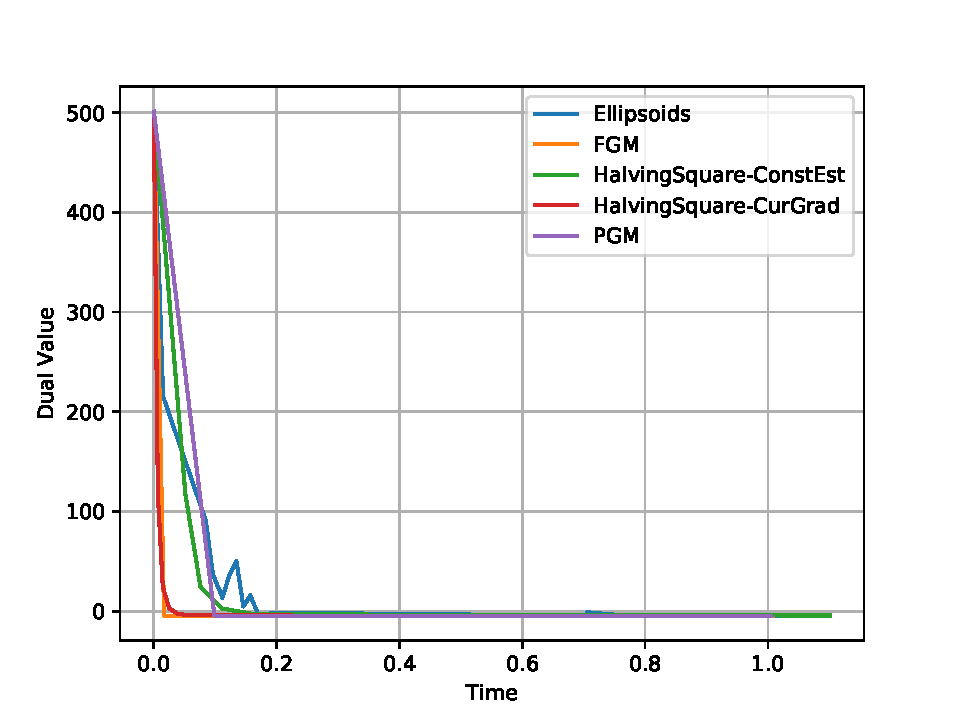
\includegraphics[width=0.25\linewidth]{Tests/Images/100_1e-03.pdf} \label{100_3} }  
\hspace{2ex}
\subfigure[]{
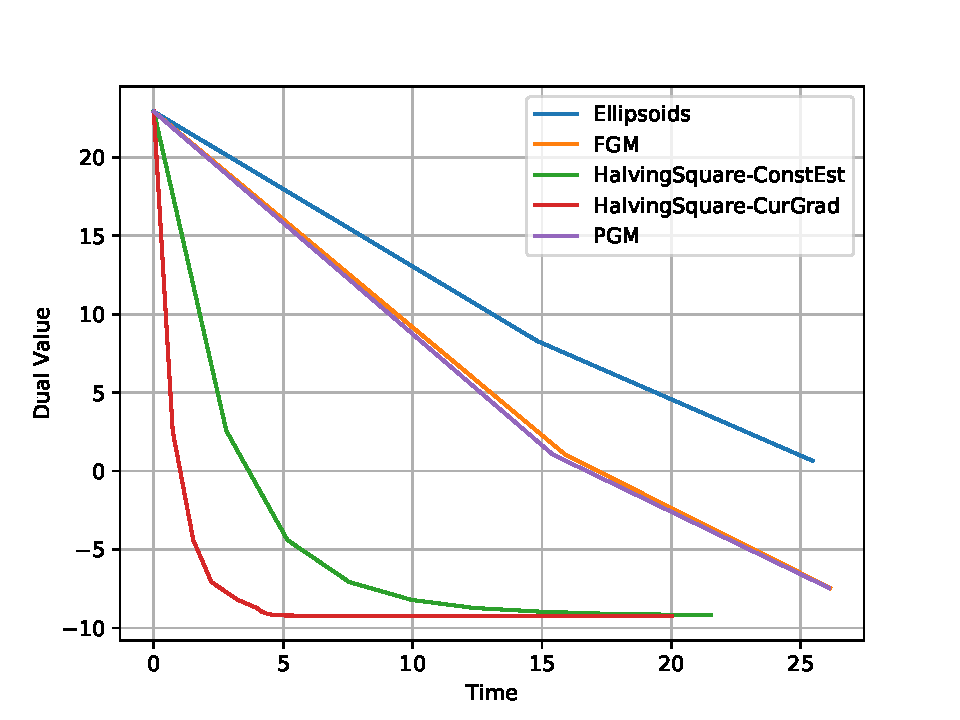
\includegraphics[width=0.25\linewidth]{Tests/Images/100_1e-10.pdf} \label{100_10} }
\vspace{2ex}
\subfigure[]{
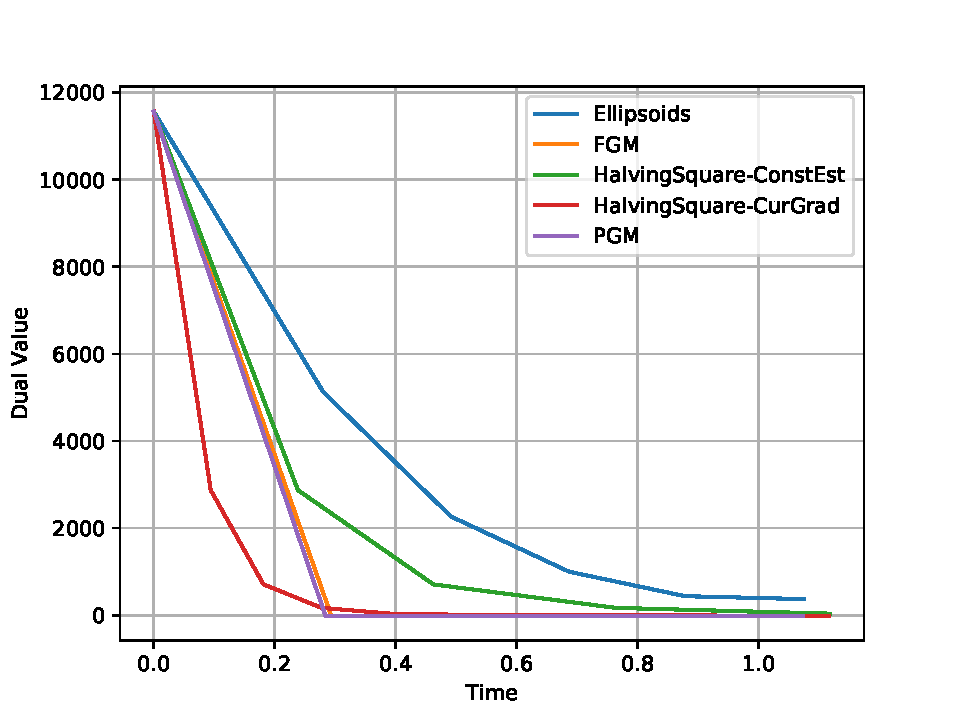
\includegraphics[width=0.25\linewidth]{Tests/Images/1000_1e-03.pdf} \label{1000_3} }  
\hspace{2ex}
\subfigure[]{
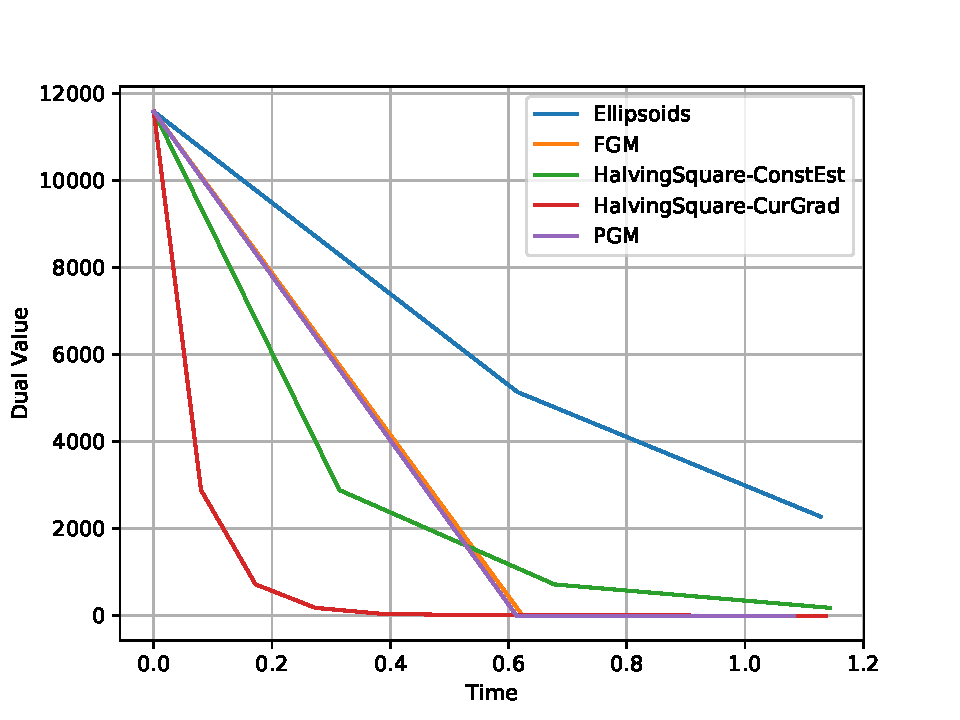
\includegraphics[width=0.25\linewidth]{Tests/Images/1000_1e-10.pdf} \label{1000_10} }
\vspace{2ex}
\subfigure[]{
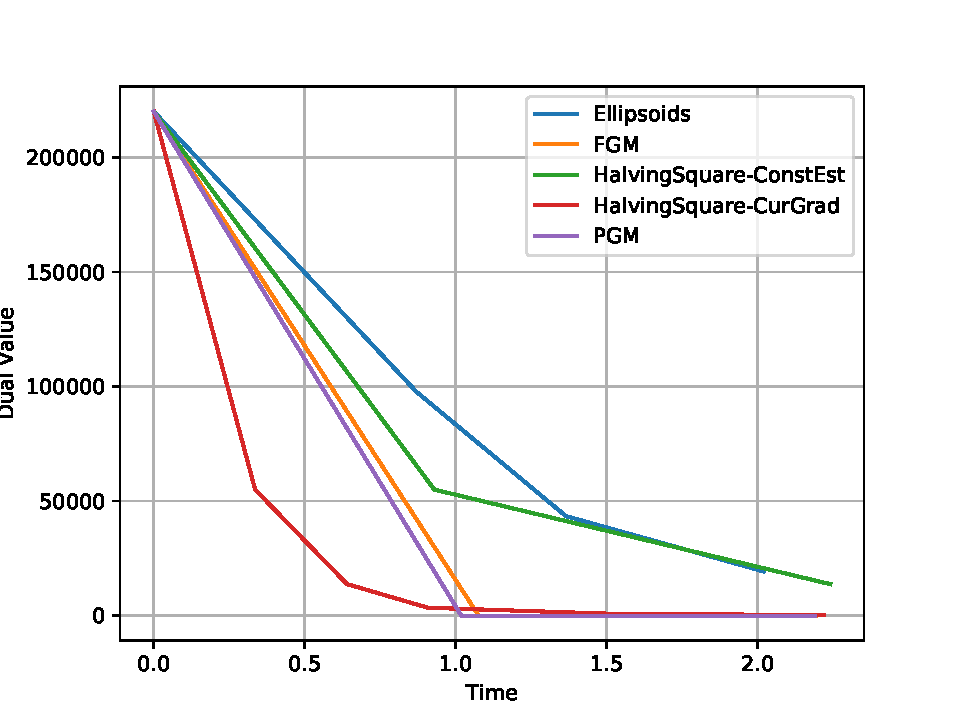
\includegraphics[width=0.25\linewidth]{Tests/Images/10000_1e-03.pdf} \label{10000_3} }  
\hspace{2ex}
\subfigure[]{
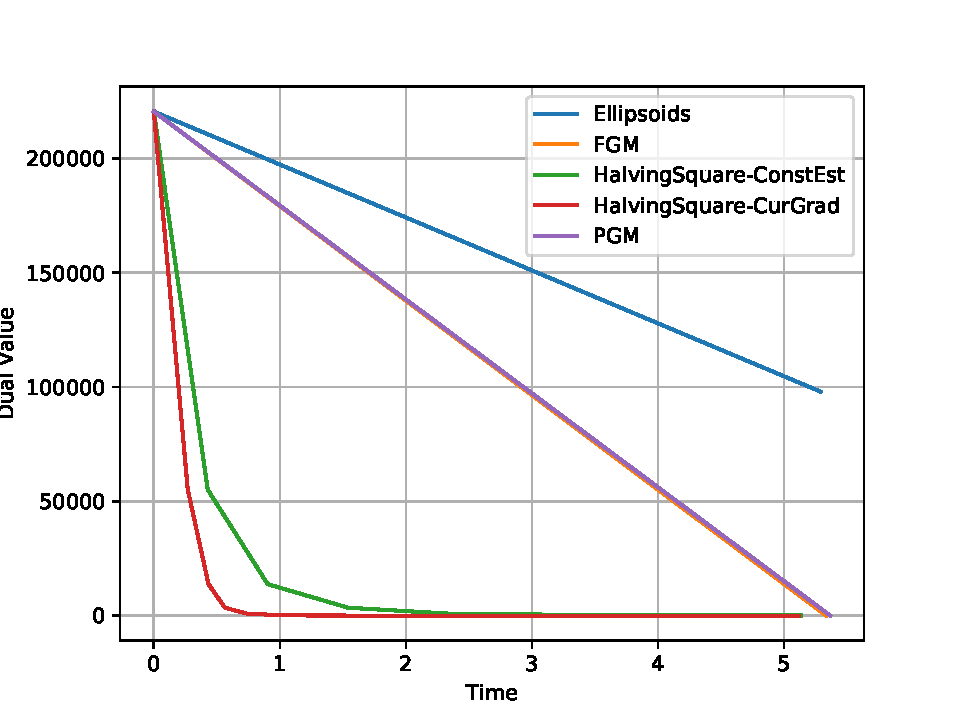
\includegraphics[width=0.25\linewidth]{Tests/Images/10000_1e-10.pdf} \label{10000_10} }
\hspace{2ex}
\caption{Comparison of different on inexact methods for task with different dimension $N$ and for different required accuracy $\epsilon$: \subref{100_3} $N=100,\epsilon=10^{-3}$; \subref{100_10} $N=100,\epsilon=10^{-10}$; \subref{1000_3} $N=1000,\epsilon=10^{-3}$; \subref{1000_10} $N=1000,\epsilon=10^{-10}$; \subref{10000_3} $N=10000,\epsilon=10^{-3}$; \subref{10000_10} $N=10000,\epsilon=10^{-10}$. } \label{fig:image}
\end{figure}

Let's compare our method with inexact ellipsoid method and gradient methods (PGM and FGM) with $(\delta, L,\mu)$ oracle (see previous subsection \ref{Inexact}) on a dual task.

For to find $\textbf{x}(\lambda)$ we will use gradient descent. There are theoretical result that can help to manange distance $\|\textbf{x}_k-\textbf{x}^*\|$ from optimal point to its current approximation. In particular, there are following results:
\begin{itemize}
\item If $f$ is a convex function with $L$-Lipschitz continious gradient then gradient descent with step $\alpha_k = \frac{1}{L}$ converges with speed
$$\|f(\textbf{x}_k)-f(\textbf{x}^*)\|\leq \frac{\|\textbf{x}_0-\textbf{x}^*\|}{k+4}$$
\item If $f$ is a $\mu$-strong convex function with $L$-Lipschitz continious gradient then gradient descent with step $\alpha_k = \frac{1}{L+\mu}$ converges with speed
$$\|f(\textbf{x}_k)-f(\textbf{x}^*)\|\leq \left(\frac{M-1}{M+1}\right)^kL\|\textbf{x}_0-\textbf{x}^*\|,$$
where $M =\frac{L}{\mu}$.
\end{itemize}

The proves for this statements one can find in many books of optimization, for example, in the book \cite{Polyak}.

We will use functions where $\mu$ is small enough. Therefore, our method for calculating $\textbf{x}(\lambda)$ will converge to solution according to the first estimate.

For all inexact method we will calculate $\textbf{x}(\lambda)$ with such accuracy as the method will converge to the solution with same for all methods accuracy $\epsilon$. For PGM, FGM and ellipsoids methods we will calculate $\textbf{x}(\lambda)$ with accuracy $\frac{\epsilon}{2}$ on function. For our method with the both strategies we will calculate $\textbf{x}(\lambda)$ untill the conditions from the \ref{dual} is approached.


We consider the following prime task:

\begin{gather}
\label{prime}
f(\textbf{x}) = \ln \left(1+\sum_{k=1}^ne^{\alpha x_k}\right) + \beta\|\textbf{x}\|_2^2\rightarrow \min\limits_{\textbf{x}\in \mathbb{R}^N}\\
g_k(\textbf{x}) = \langle \textbf{b}_k, \textbf{x}\rangle+c_k\leq0, k = \overline{1,m}\\
\end{gather}

It is task of minimization the LogSumExp-function with $l2$-regularization. The regularization parameter $\beta$ determines strong convexity of our task and in the tests one takes $beta=0.1$. The $N$ is diminsionality of primal task and is determined for different tests below. The parameter $\alpha$ is equal to 1. The parameters $c_k$ are equal to 1 too. The vectors $\{b_k\}_{k=1}^m$ are generated randomly for the each test. The $m$ is equal to dimensionality of dual task and in the current case is equal to 2.

The LogSumExp-problem is $L$-Lipschitz continious function with $M$-Lipschitz continious gradient where $L=1$ and $M=\alpha$. Therefore:
$$L_f = \alpha+2\beta R, M_f = \alpha^2 + 2\beta,$$
$$\mu_f = 2\beta,$$
where $R=\|\textbf{x}_0-\textbf{x}^*\|$ is the size of initial approximation. The functions $g_k$ are $L_k$-Lipschitz continious where $L_k=\|b_k\|$. 

We introduce the following notation:

\begin{equation}
\label{phi}
\phi(\lambda_1, \lambda_2) = -\min\limits_{\textbf{x}\in \mathbb{R}^N}\left(f(\textbf{x}) +\lambda_1 g_1(\textbf{x}) +\lambda_2g_2(\textbf{x})\right)
\end{equation}

In such notations the dual task for the task \ref{prime} looks like:

\begin{gather}
\phi(\lambda_1, \lambda_2) \rightarrow \min\limits_{\lambda_1, \lambda_2}\\
\text{s.t}\, \lambda_1, \lambda_2 \geq 0
\end{gather}
 
Obviously, $\min\limits_{\textbf{x}}f(\textbf{x}) \geq 0$. Therefore, according to \ref{restr:dual} we can add following conditions on the dual variables:

$$|\lambda_k| \leq \lambda_{\text{max}}=\frac{f(\overline{\textbf{x}})}{\gamma}, k=1,2$$

And we have following task:

$$\phi(\lambda_1, \lambda_2) \rightarrow \min_{0\leq\lambda_k\leq\lambda_{max}}$$

Calculating of function and derivatave value for such task was discussed in the section \ref{details}.

We can see on \ref{fig:image} the following results. Firstly, the halving square method with provided in this work strategy \textbf{CurGrad} are the fastest method in the most tests tests. This method can be slower than other inexact methods if dimensional of primal task is small or $\epsilon$ is big. In particular, this strategy is faster than strategy with constant estimate provided in \cite{Ston_Pas}. It proves that provided by Nesterov method with strategy through gradient is the best method for to solve two dimensional dual task of minimization. Secondly, the gain of this strategy in comparison with other method is increase when the required $\epsilon$ decrease. This fact demonstrated important advantange of this strategy: it does not depend on required accuracy strongly. So, this method with constant estimate has strong dependity on it because there is this accuracy in the constant estimate, PGM and inexact ellipsoid method require that the $x(\lambda)$ is found with accuracy depended on $\epsilon$. But halving square with ellipsoid method has not such dependety.
\section{Conclusion}

We discussed and proved that this method converges to the solution for smooth convex functon. Moreover, in the \cite{Ston_Pas} there is conterexample when the problem is non-smooth and we can not to converge to the solution with the accuracy on function better than a constant.

After it we discussed different strategy for one-dimensional task. Two strategies were considered. The both suggest to use stop conditions that are met when the current approximation is "very near" to the segment's solution. The first compares the distance between them with derivative value in accurate segment's solution but the second compares it with derivative value in approximation. In the experiment the first has a little better result but it can not be used for real task. The second strategy using derivative value in current approximation is significantly better then constant estimate and does not depend on required accuracy.

But all this strategy are good when the derivative value is high enough. But when the segment is near to the global solution this value will be small. Therefore one needs to make a lot of iterations on segment. For to avoid it we consider additional stop condition for global task on square when in current approximation the derivative value is near to zero.

The most steps of methods assumped that derivative can be calculated accurately. But the main method purpose is to solve dual problems and for it one can not usually calculate it so. That's why we consider different modifications of this method for to solve such problems. The important moment is we don't add some dependence on initial required accuracy in the modificated method.

Finally, we compared our method with new strategy for dual problem to prime LogSumExp problem with two linear constaints with our method with strategy using the constant estimate, primal gradient method and fast gradient method with $(\delta, L, \mu)$ -oracle and with inexact ellipsoids methods. The Halving Square Method is the fastest of them for enough high dimension (more 100) and for enough high required solution ($1e-3$ and more).

\newpage
\begin{thebibliography}{3}
\bibitem{task}
Gasnikov A.  Universal gradient descent // MIPT --- 2018, 240 p.
\bibitem{Ston_Pas}
Pasechnyk D.A., Stonyakin F.S.  One method for minimization a convex Lipchitz continuous function of two variables on a fixed square // arXiv.org e-Print archive. 2018. – URL: \href{https://arxiv.org/pdf/1812.10300.pdf}{https://arxiv.org/pdf/1812.10300.pdf}
\bibitem{Nesterov}
Nesterov U.E.  Methods of convex optimization // M.MCNMO --- 2010, 262 p.
\bibitem{conda}
Anaconda[site]. At available: \href{https://www.anaconda.com}{https://www.anaconda.com}
\bibitem{DDR-theorem}
Danskin, J.M.: The theory of Max-Min, with applications. J. SIAM Appl. Math.14(4) (1966)
\bibitem{Stonykin}
Fedor S. Stonyakin, Mohammad S. Alkousa, Alexander A. Titov,and Victoria V. Piskunova1 On Some Methods for Strongly Convex Optimization Problems with One Functional Constraint // ...
\bibitem{PGM}
Olivier Devolder Exactness, Inexactness and Stochasticityin First-Order Methods for Large-ScaleConvex Optimization // UCL --- 2013,
\bibitem{Ellipsoids}
Need Reference To Book with Inexact Ellipsoids
\bibitem{Polyak}
B.T. Polyak. The Introduction to Optimization // Moscow, Science - 1983
\bibitem{my_git}
Repository with code: \href{https://github.com/ASEDOS999/Optimization-Halving-The-Square}{https://github.com/ASEDOS999/Optimization-Halving-The-Square}
\end{thebibliography}
\end{document}
